%
% File: outline.tex
% Author: Oliver J. H. Feighan
% Description: Thesis outline
% Thesis outline
%
%\let\textcircled=\pgftextcircled
\chapter{Introduction}
\label{chap:intro}

\initial{P}hotosynthesis is the bedrock of life on this planet. It is often the 
first step in the food chain, establishing ecosystems from a near unlimited source 
of sunlight. The photosynthetic organisms formed around 3.5 billion years ago \cite{Blankenship2010}.
Some of the most studied organisms are
purple bacteria, \cite{Cogdell2021}. These organisms use light harvesting complexes 
(LHCs) to absorb and stabilise energy from light which is eventually transferred 
to reaction centres \cite{Klamt2008}. The mechanism for creating adenosine triphosphate
(ATP, the energy source require for biochemical processes) occurs at these reaction
centres and uses the electronic energy gathered from photons for charge transfer.
These complexes are extremely efficient, with the light harvesting complex 1 and 
2 (LH1 and LH2 respectively) found in purple bacteria being around 95\% efficient
at transferring the electronic energy to charge separation \cite{Tretiak2000}.

Many types of LHCs exist, differing by the type of chlorophyll pigments as well 
as structural features. Most often these complexes are formed of repeated units.
For example the LH2 complex found in \emph{Rhodoblastus acidophilus} is formed of 
a trimer unit with two bacterial chlorophyll \emph{a} (BChla) chromophores in close 
proximity with parallel porphyrin planes, and a third chromophore perpendicular 
at greater separation (shown in figure \ref{fig:LH2_subunit}) \cite{Cogdell2006}. 
This unit is then repeated to form a circular structure with anywhere between an
8-10 fold symmetry depending on the species of bacterium (see figure \ref{fig:LH2_rings})
\cite{Mallus2018, Cleary2013}. The efficiency of these LHCs is due to these structures,
the conformations of the chromophores, and their effect on nuanced electronic energy
transfer mechanisms \cite{Harel2012}.

\begin{figure}
	\centering 
	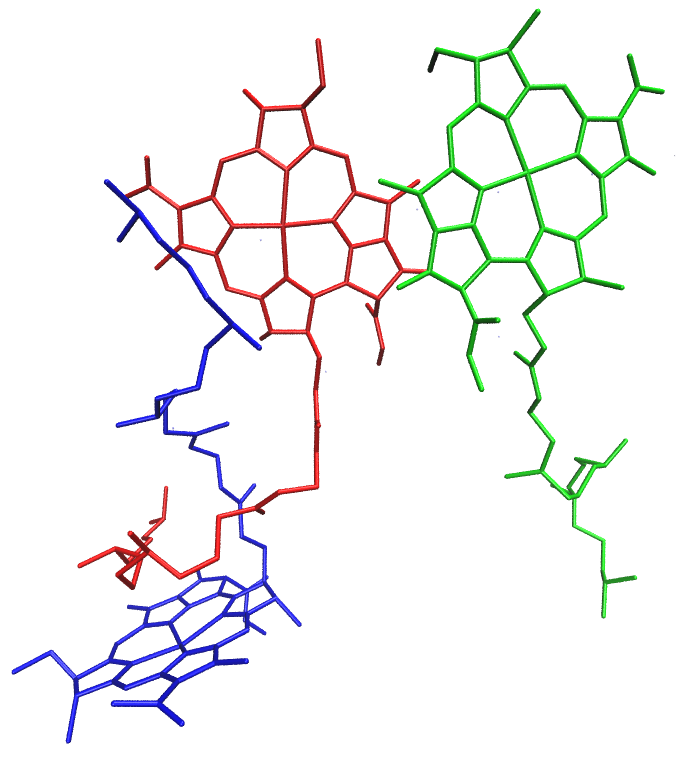
\includegraphics[scale=0.3]{chapters/1_introduction/subunit.png}
	\caption{The trimer chlorophyll unit found in LH2, coloured by ring type (red and green
	for B850a and B850b, blue for B800).}
	\label{fig:LH2_subunit}
\end{figure}

\begin{figure}
	\centering 
	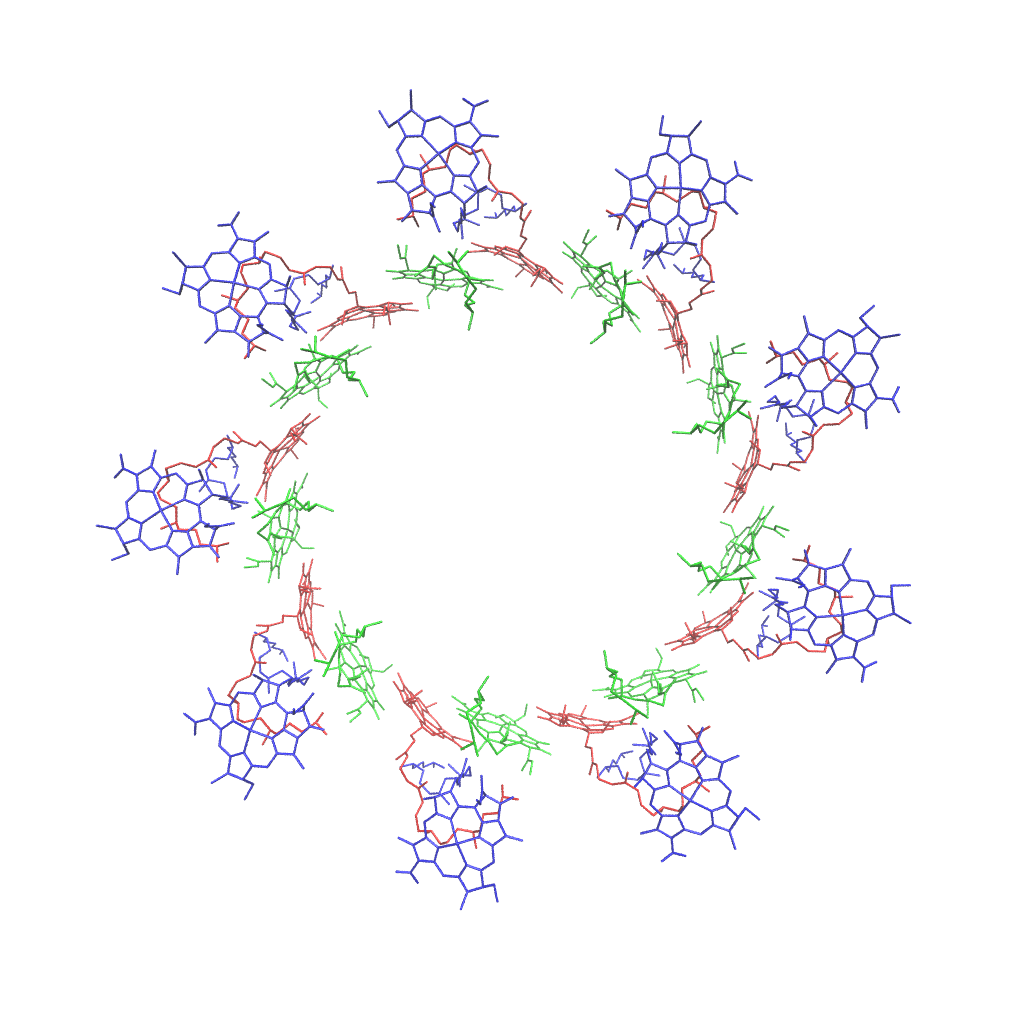
\includegraphics[scale=0.3]{chapters/1_introduction/ring_assign.png}
	\caption{The complete chlorophyll system found in LH2, coloured by ring type
	(red and green for B850a and B850b, blue for B800). This particular structure 
	has a 9-fold symmetry, giving the circular ring structures.}
	\label{fig:LH2_rings}
\end{figure}

Detailed computational study of these structures has been possible since the first
reports on high level resolution of crystal structures \cite{Mcdermott1995, Koepke1996} 
and has produced a wealth of analysis from investigations that could only be done 
with computational methods requiring the crystal structure. Many of these studies 
explore the complex mechanisms of electronic energy transfer as well as environmental 
effects of the protein scaffold on spectroscopic properties of LHCs \cite{SlaMa2020, Jang2015, Curutchet2016, Mirkovic2016}. 
These studies show that the effects of the protein which occur on the atomistic
level are an important aspect to capture in LHC models.

To investigate the efficiency of electronic energy transfer it is necessary to use 
a model for the excited states of LHCs. These models use a Hamiltonian to calculate
the states in a system, similar to many other electronic structure problems. However 
due to the size of these complexes it is usually necessary to reduce the number of 
degrees of freedom in these Hamiltonians \cite{Mallus2018, SlaMa2020}. For LH2, 
the chlorophyll molecules alone contain 3780 atoms with an additional ~6000 atoms 
for the entire scaffold \cite{Neugebauer2008, Cherezov2006}. Including a membrane 
and explicit solvent can quickly lead to system sizes in the region of 300,000 atoms \cite{Mennucci2019}.

Usual electronic structure methods that describe molecular excited states (e.g. 
DFT) are not tenable for LHCs. Instead a Frenkel-Davydov model is more appropriate
due to the weak coupling, and this model recaptures the delocalisation of excited
states over pigment sites \cite{Frenkel1931, Davydov1964}. This model constructs
the Hamiltonian from intra-site energies and inter-site interactions, reducing the
degrees of freedom of the Hamiltonian from the entire state to just single chromophores.
A more formal description is given in the next chapter.

The Frenkel exciton Hamiltonian can either be constructed from static parameters,
fited to experimental data or calculated theoretical values, or as functions of LHC 
geometry and/or time. A popular example of static parameters for LH2 was produced
by Tretiak \emph{et al.} \cite{Tretiak2000}. To recover a truly atomistic treatment
of LHCs it is necessary to take the second approach, which can be far more expensive 
to calculate as Hamiltonians are required for every frame in a time series of LHC 
geometries, explicitly treating the geometry variations. This approacg also comes 
with the caveat that methods used to construct the exciton Hamiltonian have to be
quite accurate as geometry variations are usually very small, although these small
variations are also used to justify the averaging approaches.

Often atomistic LHC models fall into a similar pattern (recently reviewed by Mennucci 
\emph{et al.})\cite{Cignoni2022}. Electronic structure calculations are used to
produce excited state properties for individual sites which in turn are used to
construct Frenkel exciton Hamiltonians, ultimately giving the excited states of
the whole LHC. The main design choices for LHC models are in choosing methods for
these steps. The first choice is which electronic structure and response method 
to use to calculate intra-site properties, and then the second choice is how to 
use these properties to construct the exciton Hamiltonian. The decisions on these
choices are highly dependent on the level of detail required for the exciton system
(atomistic or coarse grain), and the volume of unique Hamiltonians required (how 
many frames of molecular dynamics (MD) are used). For a coarse-grain model, where
the full geometry of the chlorophyll system is not important, then more approximate 
methods can be used.

For a truly atomistic approach often density functional theory (DFT) and linear 
response methods (time-dependent DFT or TD-DFT) are used to calculate single site
properties \cite{Cignoni2022}. Due to the size of chlorophyll molecules, using high
level methods such as SCS-CC2 and EOM-CCSD would not be reasonable. Even with TD-DFT
methods only a limited number of explicit Hamiltonians could be constructed before
the cost is too high. If a large number of LHC geometries need to be calculated 
then further approximations are necessary.

This trade-off between computational expense and fine-grain accuracy is the main
issue in designing physical models for the excited state of LHCs. Often it is found
that while coarse-grain models are good enough for large scale phenomena, smaller
details are lost when not using high-level electronic structure and response calculations.
Some solutions to this problem are offered in the literature which are discussed 
below, however each have limitations. These limitations sketch out the potential 
for a new kind of excited state LHC model, which is the main investigation of this
work.

\section{Efficient Response Methods}
\label{sec:efficient_response_methods}

The most obvious solution to this scaling problem is to make the electronic structure 
and response calculations more efficient, often done at the expense of accuracy.
Many recent studies use tight binding methods such as TD-DFTB or ZINDO to calculate
response properties \cite{Jurinovich2015, Olbrich2010, Curutchet2011, Curutchet2012}. 
These methods can include environmental effects (such as continuous solvent models 
or point charge embedding) and are implemented in a wide range of electronic structure
packages. Comparisons of low-level (TD-DFTB), mid-level (i.e. TD-DFT) and high-level
(multireference configuration-DFT and complete active-space SCF) methods have demonstrated
that often lower level methods are accurate enough but this is not given for every
method and so benchmarking is necessary \cite{Andreussi2015, Hansen2019, Poddubnyy2021}.

Designing tight-binding models can be challenging due to the balance between accuracy
and the parameters that need to be fit. This issue has been explored thoroughly 
by the xTB methods developed by Grimme \emph{et al.} \cite{Bannwarth2020}. A more
in-depth discussion of all of these methods is given in the next chapter, however
as their excited state method (referred to as sTDA-xTB) is relevant to the discussion
on LHC models, an outline and discussion of this method are given below.

\subsection{sTDA-xTB}
\label{subsec:stda_xtb}
sTDA-xTB ("simplified Tann-Dancoff Approximation - eXtended Tight Binding") is another
method in the family of xTB methods developed by the Grimme group and is parameterised
for transition properties \cite{Grimme2016}. The accuracy in calculating transition
energies with this method is very good with the error compared to high-level methods
such as SCS-CC2 being around 0.3 - 0.5 eV.

Similar to other xTB methods, sTDA-xTB is based on tight-binding electronic structure
that uses empirically fitted parameters and a minimal basis set. Discussed in more
detail in chapter \ref{chap:background_theory}, tight-binding schemes assume small
variations in electron density that remove the need to treat core electrons explicitly
and often only consider valence electron effects. It was trained on a set of highly
accurate coupled cluster and density functional theory excitation energies, as well
as atomic partial charges for inter-electronic interactions.

Unlike other xTB methods, coefficients in the basis set for sTDA-xTB are dependent
on coordination number of the atom centres. This makes basis functions far more 
flexible, which could only be achieved with fixed basis functions by using diffuse
or additional orbitals in the basis set. It also uses two sets of parameterized 
basis sets - a smaller valence basis set (VBS) and an extended basis set (XBS).
Whilst this approach reduces the cost of having larger basis sets, it makes calculating
the gradients of transition properties much more difficult.

The two basis sets are used to construct formally similar Fock matrix elements,
although in practice they use different global parameters. The core Hamiltonian
is similar to other DFTB methods that use a self-consistent charge (SCC) method 
to obtain molecular orbital (MO) coefficients. It is given by

\begin{equation}
\bra{\psi_\mu} H^{\text{EHT, sTDA-xTB}} \ket{\psi_\mu}= \frac{1}{2} \left(k^l_\mu k^{l'}_\nu\right) \frac{1}{2} \left(h^l_\mu h^{l'}_\nu\right) S_{\mu\nu} - k_T \bra{\psi_\mu}\hat{T}\ket{\psi_\nu}
\end{equation}
%
where $\mu,\nu,l,l'$ are orbital and shell indices, $k^l_\mu$ are shell-wise 
H{\"u}ckel parameters, $h$ are effective atomic-orbital energy levels, $S_{\mu\nu}$
is the overlap of orbitals $\mu$ and $\nu$, $k_T$ is a global constant and $\hat{T}$
is the kinetic energy operator. The charges used in the inter-electronic repulsion 
function are given by charge model 5 (CM5) \cite{Marenich2012} charges for the XBS
Fock matrix. These are calculated using Mulliken charges obtained from diagonalizing
the Fock matrix with the VBS. The charges for the initial VBS Fock matrix are based
on Gasteiger charges \cite{Gasteiger1978}, modified by the parameterized
electronegativities of atoms in the system.

The whole process for determining molecular orbitals can be summarized as:
\begin{enumerate}
	\item Calculate modified Gasteiger charges for the first initial guess
	\item Diagonalize Fock matrix in the VBS to get the first set of Mulliken charges
	\item Compute CM5 charges
	\item Diagonalize Fock matrix in the VBS again for final set of Mulliken charges.
	\item Recalculate CM5 charges with this final set, and diagonalize the Fock matrix in the XBS. 
	\item The molecular orbital coefficients from this are then fed to the response theory.
\end{enumerate}

The response theory for this method is based on previous work in the Grimme group
on the simplified Tamm-Dancoff Approximation \cite{Grimme2013}. There are several
approximations made between full linear response theory and the sTDA method. First
is the Tamm-Danncoff approximation, where some transition characters are ignored. 
The second approximation is to use a Mataga-Nishimoto-Ohno-Klopman (MNOK) method 
to calculate two electron integrals instead of explicitly calculating them \cite{Nishimoto1957, Ohno1964, Klopman1964}.

Transition charges are used to calculate these MNOK integrals. These charges $q^A_{nm}$
(centred on atom $A$ and associated with the transition $ n \rightarrow m$) are
computed using a Löwdin population analysis

\begin{equation}
q_{nm}^A = \sum_{\mu \in A} C^\prime_{\mu n} C^\prime_{\mu m}
\end{equation}

where the transformed coefficients $C^\prime_{\mu n}$ are given by orthogonalising
the original MO coefficients $\textbf{C}$

\begin{equation}
\textbf{C}^\prime = \textbf{S}^{\frac{1}{2}} \textbf{C}
\end{equation}

and $\mu$ is an index that runs over the atomic orbitals (AO). The MO coefficients
are the solution of diagonalizing the Fock matrix (from the Roothaan-Hall equations,
see equation \ref{eq:roothaan_hall}).

The approximations to full two electron integrals are given by charge-charge interaction
damped by the MNOK functions. For exchange and Coulomb type integrals different 
exponents are used along with an additional free parameter to recover the amount 
of Fock exchange mixing in the original matrix element equation. These will be discussed
in more detail in chapter \ref{chap:chl_xtb} as they are a crucial part of designing 
a new response method for chlorophyll systems.

Lastly the single particle excited space used to construct the full transitions
is truncated more than that of normal TD-DFT. This reduces the number of elements
that need to be calculated, reducing the time taken for diagonalization whilst also
capturing a broad enough spectrum of excitation energies. 

The sTDA-xTB method is reported as having excellent accuracy against benchmarked
data, and has been used to generate absorption spectra and other properties for 
large systems \cite{Grimme2016, Seibert2019, Wilbraham2018, Verma2022, HeathApostolopoulos2019}. 
At first glance, it would seem that this method would solve the issue of calculating 
many Frenkel exciton systems, however this is not supported by the data so far. 
Much of the work reporting sTDA-xTB accuracy has been performed on a range of systems,
and does not concern smaller geometry variations of a single system. The latter
is more important for LHCs, as it is the variations in chlorophyll geometries that 
cause variations in the exciton system and these are relatively small \cite{Sirohiwal2020}.
Without any indication on how accurate sTDA-xTB is for a range of conformers, it 
is difficult to say whether it would be better than previously used tight-binding 
methods. It may be better to start from methods that do have accurate correlations 
with system geometries, such as TD-DFT, and work from these to retain accuracy. 
This strategy is explored in the next section on statistical method based on high-level 
data to generate exciton Hamiltonian matrix elements.

\section{Statistical Methods}
\label{sec:stats_methods}

Making approximations in constructing the exciton framework is an alternative option
to response method approximations. One of the simplest ways of doing this is by 
using static parameters fit from experimental or calculated data \cite{Cory1998, Hu1997, Tretiak2000}. 
These are referred to as static in this work as the parameters do not vary between 
frames in a time series of LHC geometries. Using these static Hamiltonians negates
any variation in intra-chromophore or protein scaffold geometry, but can still produce
good predictions of physical phenomena.

If using a long timescale where the full conformation space is well sampled, exciton
Hamiltonians can be constructed from distributions of chromophore response properties
(i.e. excitation energies and transition densities) \cite{Stross2016}. These properties
are distributed along a normal distribution when taken from a set of uncorrelated 
structures. The mean and standard deviations can then be used to define a distribution
function which can be limitlessly sampled to construct Hamiltonians without the 
need for explicit calculations on structures. The Hamiltonians could utilise functions
that take into account inter-chromophore geometries, for example by calculating 
coupling values from a distribution function of transition dipole magnitudes, or
use distributions for all elements of the Hamiltonian matrix.

However even these methods are based on static parameters such as the mean and standard
deviation and are not functions of time. This means they would be ill-suited for
dynamic studies where structures at different times are correlated, which is an important
consideration for LH2 \cite{Papiz2003}. Recently machine-learning methods have been
reported that would give time-dependent Hamiltonians but still without the need 
for expensive calculations.

\subsection{Machine-Learning For Exciton Models}
\label{subsec:machine_learning} 

Machine-learning models have been used in many areas of computational chemistry,
especially in areas where both large amounts of data and well-defined metrics make 
it easy to train  methods \cite{Dral2020, Behler2011, Westermayr2020, Schutt2019, Sajjan2022}.
At their heart, these methods are similar to the static statistical methods that
have already been used for LH2 exciton systems, as they rely on parameters fitted to
high level data. However these models use machine-learning techniques to incorporate 
atomic geometry information so they are time dependent functions.

In 2016 H\"{a}se \emph{et al.} reported on a multi-perceptron or neural network (NN)
model that predicts the \Qy transition for chlorophyll molecules \cite{AspuruGuzik2016}.
Using this model, as well as fitted parameters for the exciton coupling, it was 
possible to calculate exciton population dynamics, as well as spectral densities
for chlorophyll sites in the FMO light harvesting complex. Similar to other models
a "Coulomb matrix" \cite{Rupp2012a, Montavon2013} is used as descriptor of the chlorophyll
systems defined as 

\begin{equation}
	M_{AB} = 
	  \begin{cases}
		\frac{1}{2} Z^{2.4} \text{ for } A = B\\
		\frac{Z_A Z_B}{\left\lvert \mathbf{R}_A - \mathbf{R}_B\right\rvert} \text{ for } A \neq B
	  \end{cases}
\end{equation}
%
where $Z_A$ is some measure of the atomic charge on atom $A$, and $R_A$ is the position
vector. It can be seen that the off-diagonal elements are simply the Coulombic interactions,
and diagonal elements are a polynomial of the atomic charges. This descriptor is
popular due to the similarity in information that an electronic structure calculation
would start from, namely the positions and nuclear charges of atoms \cite{Raghunathan2022}.

This matrix is used as an input for a neural network model. A neural network is 
a series of matrix multiplications applied to input data that overall acts as a
non-linear function. These multiplications are organised into to layers with each 
element in the output of the multiplication referred to as a node. The first and
last layers are called  input and output layers and any steps in-between referred
to as "hidden" layers \cite{Rumelhart1986}.

\begin{figure}
	\centering
	\begin{neuralnetwork}[height=4]
        \inputlayer[count=3, bias=true, title=Input\\layer]
        \hiddenlayer[count=4, bias=false, title=Hidden\\layer 1] \linklayers
        \hiddenlayer[count=3, bias=false, title=Hidden\\layer 2] \linklayers
        \outputlayer[count=2, title=Output\\layer] \linklayers
	\end{neuralnetwork}
	\caption{A schematic of a neural network showing how inputs, such as the
	(flattened) Coulomb matrix, are ordered into nodes (green and yellow) and can
	be used to generate outputs (red nodes). The blue nodes between these layers
	constitute the "hidden layers". Each arrow leading to a node represents a matrix
	multiplication and activation function application. The values in the output
	layer for models discussed in the text would be \Qy transition energies or atom
	centered transition charges.}
	\label{fig:neural_network}
\end{figure}

A layer is a distinct vector of values. For example, flattening the Coulomb matrix
into a 1D vector gives the input layer, and the \Qy transition energy is the output 
vector (of 1 element). A vector $\mathbf{V}_n$ at layer index $n$ gives the next layer
by multiplication with a coefficient matrix $c$

\begin{equation}
	\mathbf{V}_{n+1} = \mathbf{c}_n \mathbf{V}_n	
\end{equation}
%
where the coefficient matrices $\mathbf{c}_n$ are fitted to give the smallest deviations
of the output layer against target data (i.e. error in predicted \Qy energies).
Often additional functions are used to modify these values giving new vectors $\tilde{\mathbf{V}}_{n+1}$.
These also include parameters, such as linear scaling constants $m$, and the most 
common functions are sinusoidal, sigmoid, linear ($\tilde{\mathbf{V}}_{n+1}=m \mathbf{V}_{n+1}$) 
or rectified linear unit ($\tilde{\mathbf{V}}_{n+1}=\text{max}\left(0, m \mathbf{V}_{n+1} \right)$). 
NN models are conceptually similar to biological neurons which take in electrical
signals and through some mechanism can be activated to send out a different signal.
The coefficient matrices $\mathbf{c}_n$, and any other parameters in the activation
functions, are fit by a back-propagation method which also uses parameters - these
second types of parameters are referred to as hyper-parameters and have to be optimized 
to give the best coefficient matrix using supervised learning techniques such as
a systematic grid-search. Other considerations such as over-fitting also need to 
be taken into account. The brief explanation of NNs here is fairly simplistic, and
creating these models takes in-depth knowledge and experience to achieve good results.

The H\"{a}se model predicted \Qy transition energies with around a 0.3 meV error
for all of the 8 sites in the FMO complex \cite{AspuruGuzik2016}. This is exceptionally
accurate, supporting the idea that atomic positions and nuclear charges contain 
all the information necessary to predict transition energies. It is noted in this
work that the root mean squared deviations (RSMD) of Nitrogen atom positions compared 
to the energy-minimized crystal structure correlate well with excited state properties. 
This implies that structural information is key to get transition properties correct and should be
a primary consideration when discussing models for chlorophyll transition properties.
Exciton properties, such as the time series of exciton populations, were also well 
reproduced using these \Qy energies, although the coupling parameters were taken 
from other fits and not from a NN method.

Another method, developed by Farahvash \emph{et al.}, utilized both neural networks
and kernel ridge regression (KRR) to predict both site energies as well as exciton 
coupling parameters, giving a completely time dependent exciton Hamiltonian \cite{Farahvash2020}. 
KRR is another machine-learning method that can be understood as two processes \cite{Hastie2009}. 
First is the ridge regression, which is similar to a linear regression model but 
with an additional factor to account for co-linear relationships between inputs.
Regression models are multivariate linear models that follow the form

\begin{equation}
	f^\prime\left(\mathbf{X}\right) = \mathbf{X} \mathbf{\beta}
\end{equation}
%
where $f^\prime\left(\mathbf{X}\right)$ are the predicted values of some metrics $f\left(\mathbf{X}\right)$ 
(i.e. \Qy energy or exciton coupling value), $\mathbf{X}$ is the matrix of information
used to predict the value $f$ (i.e. flattened Coulomb matrix, referred to as the feature
matrix) and $\beta$ is a set of fitted coefficients that minimise the value $\left\lvert f^\prime \left( \mathbf{x}\right) - f \left(\mathbf{x}\right)\right\rvert$.
The matrix $\mathbf{\beta}$ can be found by minimising the square of this value, 
known as the least-squares method, however this can lead to expensive terms when
calculating the inner product of the feature matrix. Here the "kernel trick" is 
used to make these terms easier to calculate. This rearranges the minimisation of
regression coefficients so that the inner products are not required, but requires 
a new function that compares the similarity of features. Glossing over some derivation
details, the function $f^\prime$ becomes

\begin{equation}
	f_{\text{KRR}}^\prime = \sum^{N_x}_j \beta_j k\left(\mathbf{x}, x_j\right)
\end{equation}
%
where the $N_x$ is the size of the feature vector $\mathbf{x}$ (which in the linear
model is stacked to form the matrix $\mathbf{X}$), and $k$ is the kernel function.
Often this is a gaussian function of the feature vector

\begin{equation}
	k\left(\mathbf{x}, x_j\right) = \text{exp}\left(\frac{-\left(\mathbf{x}-x_j\right)^2}{2\sigma^2}\right)
\end{equation}
%
where $\sigma$ is a fitted parameter \cite{Rasmussen2006}. Again these parameters 
are optimised by a systematic search through values, similar to the grid search
referenced earlier.

In the Farahvash work a KRR model was developed for both the excitation energies
and exciton coupling parameters. However it was found that a NN model predicted 
exciton couplings with greater accuracy, which was attributed to the more complex 
conformational space. This NN model calculated atomic centered transition charges 
which were then used to calculate coupling elements with small error against higher 
level methods. This corroborates another study on exciton coupling methods that
argues that transition charge based methods are accurate enough for almost all needs \cite{Kenny2016}.

These machine-learning models show that it is possible to generate time and geometry
dependent functions that give either transition properties needed to construct exciton
Hamiltonians or the full Hamiltonians themselves. However there are some issues 
with this approach. In contrast to the sTDA-xTB method, machine learning models 
do not use any formalism that treats the electronic structure explicitly. This makes 
it difficult to include any other effects such as continuous solvent models or point
charge embedding that are often used in LHC quantum mechanics / molecular mechanics
(QM/MM) models. Some models do use QM/MM methods to generate training data but this
would only lead to pigeonholing the optimised model to the QM/MM system used. Additionally
they would not able to calculate any other properties than those fitted - for example
the models that return \Qy transition energies would not be able to return ground
state energies. There are some practical considerations as well when designing these
models such as the requirement of in-depth knowledge of machine-learning methods 
to retrain models. The cost of generating enough data to train these models is also
very high. For example the number of data points required to train the H\"{a}se and
Farahvash models was on the order of $10^4$ and $10^5$ respectively. In summary,
whilst these models are accurate enough to reliably make time-dependent Hamiltonians 
they are limited by both their designs and their construction cost.

\section{GPU Acceleration}
\label{sec:gpu_acceleration}

An alternative approach to these problem would be to accelerate the TD-DFT calculations.
This is possible with various established techniques such as multi-node parallelism
(an early example is parallelisation of GAMESS \cite{Fletcher2000}) but as this 
requires the exclusive use of many CPUs this is not a favourable option to take.
Instead a better approach is to use graphical processing units (GPUs), which have
been used to accelerate many different types of molecular chemistry simulations \cite{Pandey2022}. 
Programs written for GPUs can partition a limited number of basic operations over 
a massive number of parallel components, and this is exploited to parallelise the
bottleneck of expensive calculations \cite{McIntosh-Smith2013}. For TD-DFT this 
bottleneck is evaluating the electron integrals, but other examples of GPU usages 
include the large amount of operations required to calculate forces in MD simulations 
as well as the matrix multiplications of NNs discussed above \cite{Ufimtsev2008, Friedrichs2009, Wu2012}.

This approach does not require any parameter optimisation or new formalism but does
require appropriate hardware (GPU cards) and programs that can partition on GPUs
correctly. However this is a common feature on high performance computers. GPU-acceleration
has been used in many studies and is a popular way of drastically increasing system 
sizes while keeping computing time down \cite{Seritan2021}. It has been used for 
LHC study, for example a recent study that used full TD-DFT calculations to construct
Frenkel exciton Hamiltonians for every frame of an LH2 MD simulation \cite{Sisto2014a, Sisto2017}.

These models followed a similar workflow to exciton frameworks discussed above,
using transition properties on sites to evaluate Hamiltonian elements. In this case, 
all of the transition properties were calculated using TD-DFT with the $\omega\text{PBEh}$
functional and 6-31G basis set. These calculations were accelerated using GPU hardware
so they would require similar computing wall-time as the tight-binding and machine-learning
methods. Due to this acceleration it was also possible to calculate transition properties
on larger aggregates of chlorophyll molecules, such as a combination of the two 
subunits shown in figure \ref{fig:LH2_subunit}. There was an average error of 8 meV
when benchmarking the exciton framework against TD-DFT calculations on these hexamer
complexes\cite{Sisto2014a}. Absorption spectra predicted by full TD-DFT and the
exciton model were also very similar. The benefit of using a more efficient method
to calculate TD-DFT data is showcased by this method being able to calculate the
on-the-fly dynamic simulations of the exciton system. This requires the construction
of the Frenkel exciton Hamiltonian to be on the timescale of other gradient methods
(i.e. force-fields or some semi-empirical tight-binding methods).

Whilst computing the electron integral terms with GPUs requires far less computing 
time, storing these values is a major issue \cite{Sisto2014a}. This is due to the
lightweight memory restrictions on GPU cards, and even makes recalculation of some
integrals more efficient than storage. This means that a larger basis sets or more
complicated density functionals may be too expensive to use. Therefore trying to
calculate high-level data may be an issue for a more detailed study. It may be argued
that accelerating the generation of high-level data would be better done by machine-learning
methods.

\section{Alternative Approaches}
\label{sec:possible_novel_methods}

The underlying issue of LHC models is clear - the systems are too large to explicitly
calculate all transition properties required when using high level methods. Making
well- chosen approximations has found success in solving some parts of this issue
but often at some expense. The sTDA-xTB method (and other tight-binding methods) 
are efficient but are generally not accurate enough to give as reliable results 
as TD-DFT or higher-level methods. Machine-learning methods are accurate and efficient
but not extendable, use large amounts of expensive high level training data, and
require a good understanding of machine-learning methods. Accelerating calculations 
with GPUs could also be used but may still come up against memory issues which limits 
the extent of the basis set and density functional.

These shortcomings sketch out the need for a method that is efficient, accurate,
extendable, memory light and easy to reproduce. The work presented in this thesis
explore whether novel response methods in conjunction with efficient electronic 
structure methods could design a good method for LHCs models - this strategy is 
similar to the sTDA-xTB approach although with a more specialized scope. Most of
this work is based on tight-binding approaches as these fulfill most of the criteria 
set out above except accuracy, making them the optimal starting place. In order 
to assay the usability of these novel approaches it is necessary to benchmark transition 
properties against established methods (explored in chapters \ref{chap:dscf} and 
\ref{chap:chl_xtb}) as well as provide case studies of calculating full LHC models 
(chapters \ref{chap:excitons} and \ref{chap:LH2}). A description of all of the common 
theories used (DFT, DFTB/xTB, TD-DFT and Frenkel-Davydov models) is given in the 
next chapter.